% 物理学会講演概要集原稿用テンプレート
%		by Hitoshi Nakahara, nakahara@nuqe.nagoya-u.ac.jp
%		Created: 2004/1/7
%		Last Modified: 2004/1/15
%
% ※ 本ファイルの配布、改変等は自由に行っていただいて構いません。
% ※ 作者は本ファイルの動作を保証するものではありません。
% ※ 自らの責任に於いて使用してください。
% ※ 内容に関する質問にはお答えできないことがあります。

\documentclass[12pt, a4paper]{jarticle}
%\usepackage{citesort}
\usepackage{amssymb}
\usepackage[dvipdfmx]{graphicx}		% 図を入れるときに使用
\usepackage{wrapfig}		% 図の周りに本文を流し込みたいときに使用
\usepackage{subfigure}
\usepackage{here}
% 使用例
% \begin{wrapfigure}{r}{8cm}
% \includegraphics[width=8cm]{apparatus.eps}
% \caption{これは図のキャプションです。}
% \end{wrapfigure}
% 流し込みたい段落が続く...

%%%%% 以下のヘッダ項目を変更してください (前後に余分なスペースは入れないでください)
%% 必要に応じて改行 "\\" 等のコマンドを含めて構いません

\newcommand{\講演番号}
{14pPSA-18}

\newcommand{\講演題目}
{Mg-LPSOのL\mbox{\boldmath $1_2$} クラスターの第一原理計算}

\newcommand{\英文題目}
{First principle calculations of L12 Cluster in Mg-Zn-Y alloy}

\newcommand{\和文所属}
{関西学院大・理工}

\newcommand{\和文氏名}
{西谷滋人, 清原資之, 森下慎也}

\newcommand{\英文所属}
{Department of Informatics, Kwansei Gakuin Univ}

\newcommand{\英文氏名}
{S. R. Nishitani, M. Kiyohara, S. Morishita}

%% ヘッダ項目、ここまで

%%%%% 新規変数の定義、変更しないでください
\newlength\題目幅
\newlength\ヘッダ項目間隔
\newlength\所属インデント
\newlength\和文氏名インデント
\newlength\英文氏名インデント
\newlength\最小所属氏名間隔
\newlength\ヘッダ行間隔
\newlength\本文行間隔
\newlength\上端余白
\newlength\左端余白
\newlength\idWidth
\newlength\titleNoSpacing
\newlength\autherWidth
\newlength\affilWidthJ
\newlength\affilWidthE
\newcount\crAuthorJ
\newcount\crAuthorE
\newcount\和文氏名を右揃
\newcount\英文氏名を右揃

%%%%% 以下の数値は適宜変更してください
\setlength\題目幅{127mm}				% 題目の幅、125〜130mmが適切です
\setlength\所属インデント{17mm}			% 左端から所属を開始する位置までの長さ、15〜20mmが適切です
\setlength\和文氏名インデント{55mm}		% 和文氏名の開始位置 (所属インデント位置からの長さ)
%\setlength\和文氏名インデント{5mm}		% 和文氏名の開始位置 (所属インデント位置からの長さ)
\setlength\英文氏名インデント{55mm}		% 英文氏名の開始位置 (所属インデント位置からの長さ)
\setlength\最小所属氏名間隔{1ex}			% 氏名と所属の間の最小間隔 (これ以下になると氏名を改行します)
\setlength\ヘッダ行間隔{6mm plus .3mm minus .3mm}		% ヘッダ項目の行間、6〜7mmが適切です
\setlength\ヘッダ項目間隔{1.5mm}						% ヘッダ項目間に追加する間隔、1〜2mmが適切です
\setlength\本文行間隔{7.5mm plus .5mm minus 1mm}		% 本文の行間、7〜8mmが適切です
\setlength\上端余白{12mm}							% 出力機器に依存します
\setlength\左端余白{16.5mm}							% 出力機器に依存します
\和文氏名を右揃 = 1				% 和文氏名を右寄せにするときは1、インデント位置に揃えるときは0
\英文氏名を右揃 = 1					% 英文氏名を右寄せにするときは1、インデント位置に揃えるときは0

%%%%% ここから本文入力位置までは通常は変更の必要はありません

\setlength{\textwidth}{168mm}	% 印刷領域の幅
\setlength{\textheight}{254mm}	% 印刷領域の高さ
\setlength{\topmargin}{-1in}
\setlength{\headheight}{0mm}
\setlength{\textfloatsep}{4mm}	% 図と文章のマージン
\setlength{\idWidth}{30mm}		% 講演番号の幅
\crAuthorJ = 0
\crAuthorE = 0

%%%%% 必要な間隔を計算
\setlength{\headsep}{\上端余白}
\setlength{\oddsidemargin}{-1in}
\addtolength{\oddsidemargin}{\左端余白}
\setlength{\evensidemargin}{\oddsidemargin}
\setlength{\titleNoSpacing}{\textwidth}
\addtolength{\titleNoSpacing}{-1\idWidth}
\addtolength{\titleNoSpacing}{-1\題目幅}
\setlength{\autherWidth}{\textwidth}
\addtolength{\autherWidth}{-1\所属インデント}

% 動的に決まる長さを計算
\setbox0 = \hbox{\和文所属}
\setlength{\affilWidthJ}{\wd0}
\setbox1 = \hbox{\英文所属,}
\setlength{\affilWidthE}{\wd1}
\addtolength{\affilWidthJ}{\最小所属氏名間隔}
\addtolength{\affilWidthE}{\最小所属氏名間隔}
\ifdim\affilWidthJ<\和文氏名インデント
\addtolength{\和文氏名インデント}{-1\wd0}
\else
\crAuthorJ = 1	% 所属が長いときは氏名の前で改行
\fi
\ifdim\affilWidthE<\英文氏名インデント
\addtolength{\英文氏名インデント}{-1\wd1}
\else
\crAuthorE = 1	% 所属が長いときは氏名の前で改行
\fi

%%%%% その他の設定
\renewcommand\refname{\vspace{-15mm}}		% 参考文献のタイトルは表示はしない

% ドキュメント開始、ヘッダ項目の表示
\begin{document}
\thispagestyle{empty}
\pagestyle{empty}


\setlength\parindent{0mm}
\vrule width 0mm height 6mm depth 5mm				% タイトルの高さをキープするためのダミー
\parbox{\idWidth}{\setlength\baselineskip{\ヘッダ行間隔}
{\hfil\small\tt\講演番号\hfil}}\hspace{\titleNoSpacing}%
\parbox{\題目幅}{{\fontsize{16pt}{0pt}\selectfont{\bf\講演題目}}}\par


\vspace{\ヘッダ項目間隔}\hspace*{\所属インデント}%
\parbox{\autherWidth}{\setlength\baselineskip{\ヘッダ行間隔}
{\bf{\fontsize{14pt}{0pt}\selectfont{\和文所属}}}%
\ifnum\crAuthorJ = 0
\ifnum\和文氏名を右揃 = 0
\hspace{\和文氏名インデント}{\bf{\fontsize{14pt}{0pt}\selectfont{\和文氏名}}}%
\else
\hfill{\和文氏名}%
\fi
\else
\ifnum\英文氏名を右揃 = 0
\\\hspace{\和文氏名インデント}{\bf{\fontsize{14pt}{0pt}\selectfont{\和文氏名}}}%
\else
\\\hfill{\bf{\fontsize{14pt}{0pt}\selectfont{\和文氏名}}}%
\fi
\fi
}\par

\vspace{\ヘッダ項目間隔}\hspace*{\所属インデント}%
\parbox{\autherWidth}{\setlength\baselineskip{\ヘッダ行間隔}{\bf{\fontsize{14pt}{0pt}\selectfont{\英文題目}}}}\par

\vspace{\ヘッダ項目間隔}\hspace*{\所属インデント}%
\parbox{\autherWidth}{\setlength\baselineskip{\ヘッダ行間隔}
{\it{\fontsize{14pt}{0pt}\selectfont{\英文所属}}},%
\ifnum\crAuthorE = 0
\ifnum\英文氏名を右揃 = 0
\hspace{\英文氏名インデント}{\bf{\fontsize{14pt}{0pt}\selectfont{\英文氏名}}}%
\else
\hfill{\bf{\fontsize{14pt}{0pt}\selectfont{\英文氏名}}}%
\fi
\else
\ifnum\英文氏名を右揃 = 0
\\\hspace{\英文氏名インデント}{\bf{\fontsize{14pt}{0pt}\selectfont{\英文氏名}}}%
\else
%\\\hfill
\\{\bf{\fontsize{14pt}{0pt}\selectfont{\英文氏名}}}%なぜかここ動いてる
\fi
\fi
}\par



\setlength\parindent{1zw}\setlength\baselineskip{\本文行間隔}
\vspace*{\本文行間隔}
\vspace{-1.1\baselineskip}

%%%%% 以下の部分に本文を入力してください %%%%%
\paragraph{背景}
LPSO 構造の生成機構について,我々は「積層欠陥部に$L1_2$クラスターが形成され,そこから排斥されたZn, Yが,新たな$L1_2$クラスターを形成する」というシナリオを立てた\cite{sakamoto1}.従来の研究では,$L1_2$クラスターから1層ずつ離れたそれぞれの位置に孤立した溶質原子,あるいはZn--Yペアを挿入して第一原理計算をおこない,系全体のエネルギーの違いを比較した.系全体のエネルギーは溶質原子と$L1_2$クラスターとの距離が遠いほど単調に減少した.しかし,それは中周期的に溶質原子が濃化するという予想に反する結果であった.本研究では,これまで考慮してきたサイズより大きな溶質原子の集団を挿入することで再度検証をおこなった.
\vspace{-0.8\baselineskip}
\paragraph{手法}
坂本がhcp構造に$L1_2$クラスターを導入した際に,VASPによる構造緩和から予測された$L1_2$クラスターが2つに分離したsmall\_clusterに着目した\cite{sakamoto2}.このサイズは実験的には奥田らによって報告されているクラスターサイズに近い\cite{okuda}.
\vspace{-0.3\baselineskip}



\begin{figure}[H]
 \begin{minipage}{0.5\hsize}
  \begin{center}
   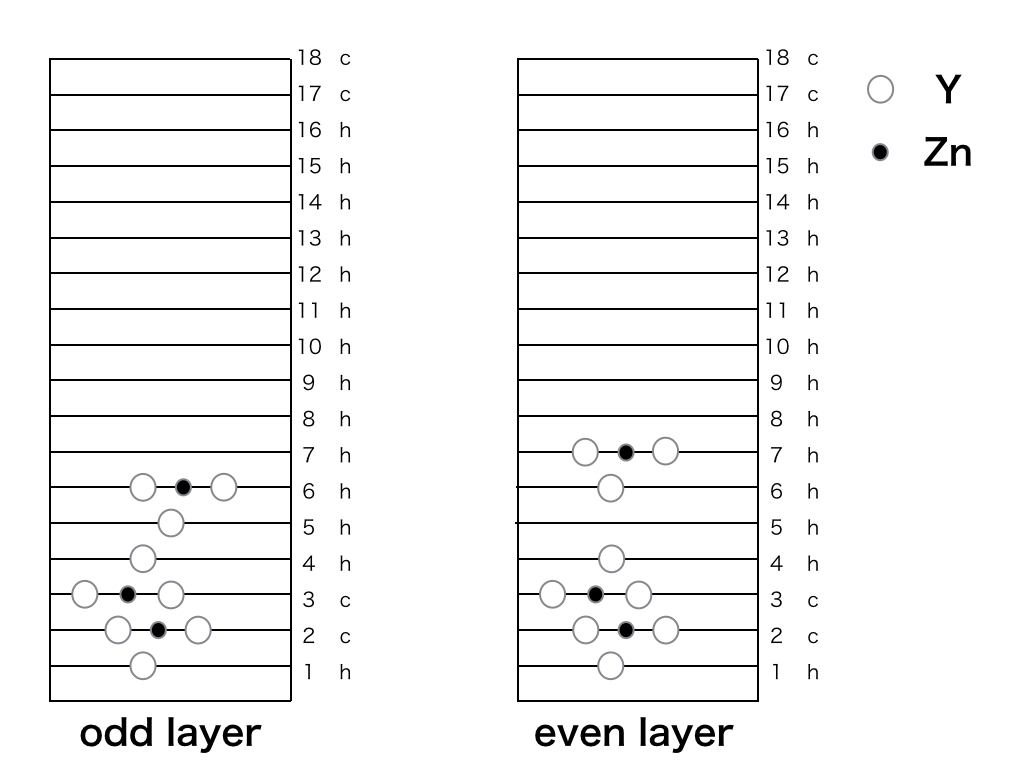
\includegraphics[width=60mm]{./small_cluster_slab.png}
  \end{center}
  \caption{今回使用した計算モデルの模式図.}
  \label{fig:one}
 \end{minipage}
 \begin{minipage}{0.5\hsize}
  \begin{center}
   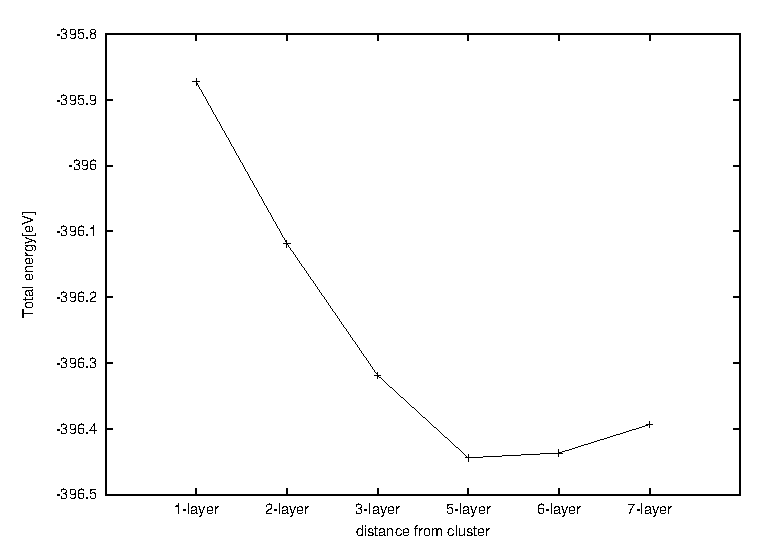
\includegraphics[width=60mm]{./small_cluster.eps}
  \end{center}
  \caption{$L1_2$クラスターから1層ずつ離れた層に溶質原子を挿入したモデルに対して第一原理計算をおこなった結果.}
  \label{fig:two}
 \end{minipage}
\end{figure}

\vspace{-1.3\baselineskip}
\paragraph{結果}
まず,$L1_2$クラスターがどのように分離した時に最も安定な構造をとるかを,small\_clusterの生成エネルギーを比較することで確かめた.幾何学的な可能性として考えやすい,上下および左右に分割した際のsmall\_clusterの生成エネルギーを比較した.その結果,上下に分割した際のsmall\_clusterの生成エネルギーの方が低く安定構造をとっているという結果が得られた.上下に分割したsmall\_clusterを積層欠陥にある$L1_2$クラスターから離れた位置へ図\ref{fig:one}に示したように挿入した. 第一原理計算によって得られた系全体のエネルギーを図\ref{fig:two}に示した.4層離れた位置での計算についてはエネルギーの値が収束せず得る事ができなかったが,他の層の計算結果から距離が離れる毎に単調減少を示すことが推測できた.

{\small\setlength\baselineskip{10pt}	% 参考文献は小さめの文字で行間を詰めてある
\begin{thebibliography}{9}
\bibitem{sakamoto1}Y. Sakamoto, C. Shirayama, Y. Yamamoto, R. Kubo,M. Kiyohara, and S. R. Nishitani: Mater.Trans., 56(2015), 933.-$>$should be PRICM
\bibitem{sakamoto2} should be PRICM
\bibitem{okuda}H. Okuda, M. Yamasaki, Y. Kawamura, M. Tabuchi, H. Kimizuka: Scientic Reports 5 (2015), 14186.
\end{thebibliography}
}

\end{document}
